%\documentclass[a4paper,11pt]{article}
%%\documentclass[11pt, oneside]{article} 
%% MNRAS is set in Times font. If you don't have this installed (most LaTeX
%% installations will be fine) or prefer the old Computer Modern fonts, comment
%% out the following line
%%\usepackage{txfonts}
%%\usepackage{newtxtext,newtxmath}
%% Depending on your LaTeX fonts installation, you might get better results with one of these:
%%\usepackage{mathptmx}
%%\usepackage{txfonts}
%
%% Use vector fonts, so it zooms properly in on-screen viewing software
%% Don't change these lines unless you know what you are doing
%\usepackage[T1]{fontenc}
%\usepackage{ae,aecompl}
%\usepackage[caption=false,font=footnotesize]{subfig}
%\usepackage{natbib}
%
%
%%%%%% AUTHORS - PLACE YOUR OWN PACKAGES HERE %%%%%
%
%% Only include extra packages if you really need them. Common packages are:
%\usepackage{graphicx}	% Including figure files
%\usepackage{amsmath}	% Advanced maths commands
%\usepackage{amssymb}	% Extra maths symbols
%
%
%
%\def\lesssim{\mathrel{\hbox{\rlap{\hbox{\lower5pt\hbox{$\sim$}}}\hbox{$<$}}}}
%\def\gtrsim{\mathrel{\hbox{\rlap{\hbox{\lower5pt\hbox{$\sim$}}}\hbox{$>$}}}}
%\def\mnras{MNRAS}
%\def\apj{ApJ}
%\def\apjl{ApJL}
%\def\aj{AJ}
%\def\planss{Planet.~Space Sci.}
%\def\prd{Phys.~Rev.~D}
%\def\apjs{ApJS}
%\def\aap{A\&A}
%\def\nat{Nature}
%\def\apss{Ap\&SS}
%\def\lcdm{$\Lambda$CDM }
%\def\hMpc{h^{-1} \text{Mpc}}
%\def\rgm{r_{\rm gm}}
%\def\hMsun{h^{-1}M_\odot}
%
%\def\xigg{\xi_{\rm gg}}
%\def\xigm{\xi_{\rm gm}}
%\def\ximm{\xi_{\rm mm}}
%\def\Omegam{\Omega_{\rm m}}
%\def\kms{\text{kms}^{-1}}
%
%\newcommand{\ef}[2]{e^{#1}_{\phantom{p}#2}}
%\newcommand{\einv}[2]{e_{#1}^{\phantom{p}#2}}
%
%
%%\voffset=-0.69in
%%\hoffset=0.12in
%

\section{Separate Universe Approach}

\subsection{Fermi Normal Coordinates}
Here I would like to reserve the separate universe equations. It will be similar to Baldauf. 


Fermi normal coordinate reference include Chp.~ 13 of \cite{misner1973gravitation}, Chp.~1 of \cite{poisson2004relativist} the \cite{manasse1963fermi}
Transport the tetrad $e^a_{\;A}$ along the geodesic $\gamma$, such that  $e^a_{\;\;0}=u^{a}(\tau)$, where $\mathbf{u}=d\gamma/d\tau$. And
\begin{align} 
g_{ab} e^a_{\;\;A}e^b_{\;\;B}= \eta_{AB} ~.
\end{align} 

\begin{align} 
\grad_\mathbf{u} e_A= u^a\nabla_a e^b_{\;\; A} = - u^a \Omega_c^{\;\; b} e^c_{\;\; A}~, 
\end{align} 
where $\Omega^{ab}=a^au^b - a^bu^a + u_c\omega_d \epsilon^{cdab}$. In the absence of acceleration and rotations the above equation gives 
\begin{align} 
 u^a\nabla_a e^b_{\;\; A}=0~.
 \end{align} 

\subsection{Power Spectrum Response}  

\begin{figure}[!ht]
 \centering
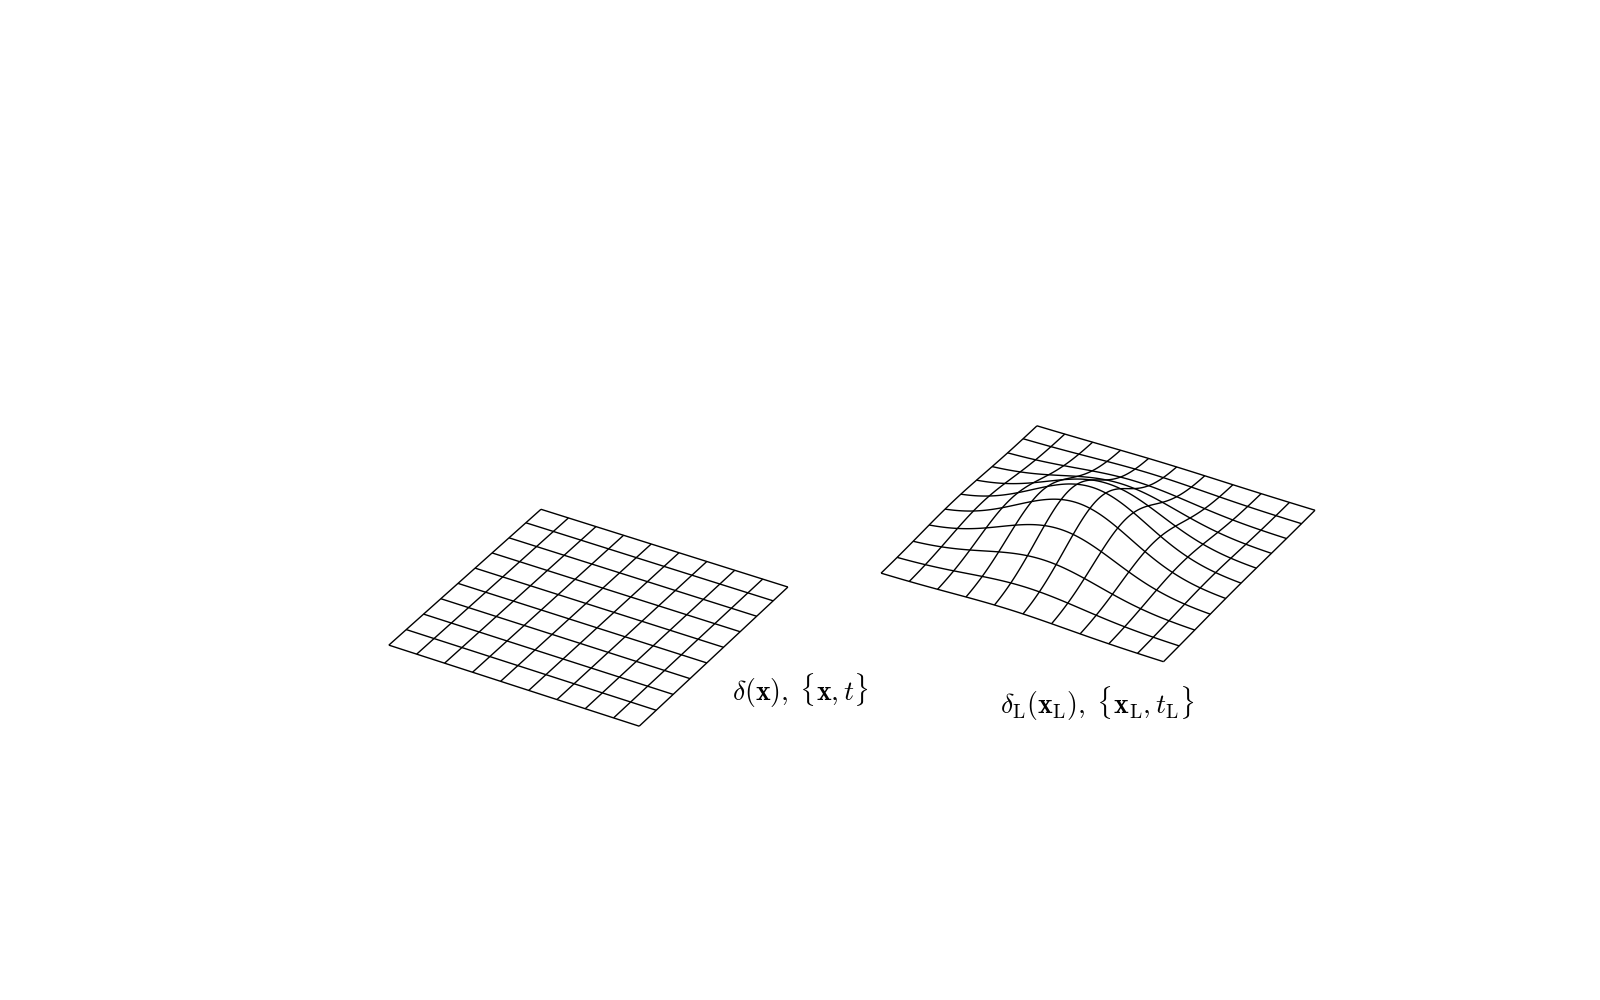
\includegraphics[width=1\textwidth]{manifolds.png}
  \caption{Illustration of the difference in correlations functions. The difference in any correlation (in real or Fourier space) is defined as difference in correlates on two different manifolds. The computation requires the appropriate mapping between manifolds. }
\label{fig:manifolds}
\end{figure}

The response of correlation function to a $\bar{\delta}$ is computed by 
\begin{align} 
\label{corr_response}
\frac{d \xi(r,t)}{d \bar{\delta}}= \frac{ \Phi[ \xi_\text{L}(r_\text{L},t_\text{L})]- \xi(r)}{\bar{\delta} } ~,
\end{align} 
where $\Phi$ is the mapping from the L universe to the ``standard" universe. The mapping is as follows 
 \begin{align} 
\begin{split} 
\xi_\text{L}(r_\text{L}, t_\text{L}) &= \langle \delta_\text{L} | \delta_\text{L} \rangle_{r_\text{L},t_\text{L}} \\
& =  \langle \delta (1+ \bar{\delta} ) + 1 | \delta(1+ \bar{\delta} ) + 1  \rangle_{r + \bar{\delta}/3,t_\text{L}} \\
& = \langle \delta | \delta \rangle_{r + \bar{\delta}/3,t_\text{L}} + 2 \bar{\delta} \langle \delta | \delta \rangle_{r + \bar{\delta}/3,t_\text{L} }+ \mathcal{O}(\bar{\delta}^2) \\
& = \xi(r + \bar{\delta}/3,t_\text{L}) + 2 \bar{\delta}\xi(r + \bar{\delta}/3,t_\text{L})  \\
& = \xi(r, t_\text{L}) + \frac{ \bar{\delta} }{3}r \partial_r \xi(r,t_\text{L}) + 2 \bar{\delta} \xi(r, t) + \mathcal{O}(\bar{\delta}^2) ~.
\end{split} 
\end{align} 
where the subscripts in the first few lines represent the position and time arguments. Plugging back into Eqn.~\ref{corr_response} gives 
\begin{align}  
\frac{d \xi(r,t)}{d \bar{\delta}} =\frac{ \xi(r, t_\text{L}) + \frac{ \bar{\delta} }{3}r \partial_r \xi(r,t_\text{L}) + 2 \bar{\delta} \xi(r, t) - \xi(r,t)}{\bar{\delta}} ~. 
\end{align} 
I have not transformed the time coordinate. I will do this later. For the linear and SPT power spectrum, the time coordinate transformation will correspond to change in the growth factor. 
The derivative term in Fourier space is computed as follows:
\begin{align} 
\begin{split} 
r \partial_r \xi(r) & =r\hat{r} \cdot \mathbf{\nabla} \xi(r) = \hat{r} \cdot  \mathbf{\nabla}  \int \frac{d^3 \mathbf{k}}{(2 \pi)^3} e^{i \mathbf{k} \cdot \mathbf{r} } P(k) \\
& = r\hat{r} \cdot \int \frac{d^3 \mathbf{k}}{(2 \pi)^3} ~i \mathbf{k}~ e^{i \mathbf{k} \cdot \mathbf{r} } P(k) \\
& = \int \frac{d^3 \mathbf{k}}{(2 \pi)^3} ~i \mathbf{r}~ e^{i \mathbf{k} \cdot \mathbf{r} } \cdot \mathbf{k}P(k) \\
& = \int \frac{d^3 \mathbf{k}}{(2 \pi)^3} ~\mathbf{\nabla}_\mathbf{k}~ e^{i \mathbf{k} \cdot \mathbf{r} } \cdot \mathbf{k}P(k) \\
& =- \int \frac{d^3 \mathbf{k}}{(2 \pi)^3} e^{i \mathbf{k} \cdot \mathbf{r} }   ~\mathbf{\nabla}_\mathbf{k}~\cdot [\mathbf{k}P(k) ]\\
& =- \int \frac{d^3 \mathbf{k}}{(2 \pi)^3} e^{i \mathbf{k} \cdot \mathbf{r} }  [ 3 P(k) + k \frac{d P(k)}{d k}] ~.
\end{split} 
\end{align} 
Therefore the power spectrum response is 
\begin{align} 
\frac{ d P(k)}{d \bar{\delta}}=  \frac{1}{\bar{\delta} }\left[ P(k,t_\text{L}) - \frac{\bar{\delta}}{3} [ 3P(k,t_\text{L} )+ k \frac{d P(k)}{dk}] + 2 \bar{\delta} P(k, t_\text{L}) - P(k,t)\right] ~. 
\end{align} 

\subsection{Linear power spectrum response} 
Linear growth factors in the L universe compared to the ``standard" universe are 
\begin{align} 
G_\text{L}( a[ 1 - \frac{1}{3} \bar{\delta} ]) = G(a)\left[ 1 + \frac{13}{21} \bar{\delta} \right]~. 
\end{align} 

To relate the linear power spectrum at time $t_\text{L}$ to time $t$ requires the ratio of growth factors squared and we have 
\begin{align} 
P_\text{lin}(k, t_\text{L})= \left[ 1 + \frac{26}{21} \bar{\delta}\right] P(k, t) 
\end{align} 

Plugging the above back into the master equation for power spectrum response gives 
\begin{align}
\frac{ d P(k)}{d \bar{\delta}} = \frac{68}{21} P(k) - \frac{1}{3} [ 3 P(k) + k \frac{d P(k)}{dk} ] ~. 
\end{align} 

\subsection{1 -loop perturbation theory}
The 1-loop growth factor relation is 
\begin{align}
P_{1-loop}(k,z)= G^2 P_{11}(k) + G^4 [P_{22}(k) + P_{13}(k)] ~, 
\end{align} 
So the transformation is 
\begin{align} 
P_{1-loop}(k,t_\text{L})=  \left[ 1 + \frac{26}{21} \bar{\delta}\right] P_{11}(k,t) +  \left[ 1 + \frac{52}{21} \bar{\delta}\right] [ P_{22}(k,t) + P_{13}(k,t) ] ~.
\end{align} 
Plugging into the master equation gives 
\begin{align} 
\frac{ d \log P(k)}{d \bar{\delta}}=\frac{68}{21} - \frac{1}{3} \frac{ d \log k^3 P(k)}{d \log k} + \frac{26}{21} \frac{P_{22}(k) + P_{13}(k)}{P(k)} ~, 
\end{align} 


